\documentclass{ltjsarticle}

\usepackage{luatexja}
\usepackage{graphicx}
\usepackage[colorlinks=true,linkcolor=blue,citecolor=blue,urlcolor=blue]{hyperref}
\usepackage{xcolor}

\usepackage{amsmath}
\numberwithin{equation}{section} % 数式番号をセクションごとに分ける


\usepackage[most]{tcolorbox}
\newtcolorbox{eqbox}[1]{%
  enhanced,
  colback=white, colframe=black,
  boxrule=0.4pt, arc=6pt,
  left=8pt, right=8pt, top=8pt, bottom=8pt, % 余白
  title={#1},                 % ← 引数がタイトルになる
  fonttitle=\bfseries,        % タイトルの体裁
  coltitle=black,
  colbacktitle=gray!10,       % タイトル帯の背景色(要らなければ white)
  attach boxed title to top left={yshift=-2mm, xshift=6pt}, % 箱内の左上に配置
  boxed title style={sharp corners, boxrule=0pt}, % タイトル枠線なし
}


\title{日本語のLaTeX入門}
\author{あなたの名前}
\date{\today}

\begin{document}

\maketitle

% 目次
\tableofcontents

\section*{前書き}
 以下の内容は、主に

\cite{a} Francis F. Chen, "Introduction to Plasma Physics and Controlled Fusion"\par
\cite{b} 宮本健郎 『プラズマ物理の基礎』\par
\cite{c} EMANの物理学\\
を参照している。





\section{プラズマとは}
\subsection{自然界でのプラズマ}
 物質の温度を上げていくと、固体、液体、気体と相変化し、さらに温度を上げると、気体分子は原子から電子が剥ぎ取られ、プラスの電荷を持ったイオンと負の電荷を持った電子とが混じった気体になる。このような高温の電離ガス状態を\textcolor{red}{プラズマ}という。
固体、液体、気体と並んで、「第四の状態」と呼ばれることもある。

 一般的に、プラズマは真空中にしか存在しない。なぜなら、空気がプラズマを冷やし、イオンと電子を再び結合させるからである。自然界においては、宇宙空間は密度がかなり低いが一種のプラズマだし、
点灯中の蛍光灯の中やロウソクの炎などは全ての原子から電子が剥がれるほどではないがこれも一種のプラズマだし、さらにオーロラや電離層もプラズマだし、冬場に体験する静電気の放電や、溶接工事に使う電気放電、落雷などもプラズマである。太陽もまたプラズマの塊である。実に、この宇宙の99\%以上の場所がプラズマであって、地球のようなそうでない場所の方が珍しいくらいである。

 Saha方程式では、熱平衡状態にある気体において、イオン化の割合を教えてくれる。

\begin{eqbox}{Saha方程式}
\begin{equation}
\frac{n_i}{n_n} \approx 2.4 \times 10^{21} \frac{T^{3/2}}{n_i} e^{-U_i/KT} 
\end{equation}  
\end{eqbox}

ここで$n_i$はイオン化された原子の密度$[m^{-3}]$、$n_n$は原子の密度であり、$K$はボルツマン定数、$U_i$は気体のイオン化エネルギーである。

(1.1)式から、$T$が大きくなるにつれて$n_i$の割合が増える、つまり気体がプラズマ状態になることがいえる。これがプラズマが高温でのみ存在する理由である。

Saha方程式の物理的な意味を指摘すると、気体中の原子は熱エネルギーに分布があり、たまたま十分大きいエネルギーの衝突を受けると電子が飛び出して電離する。低温ではそのような“速い原子”は少なく、電離はまれ。Saha式の 
$\exp{(-U_i/KT)}$は「速い原子の数が温度に対して指数関数的に減る(=低温で急減)」ことを表す。また、いったん電離しても、電子と出会えば再結合して中性に戻る。つまり、再結合率は電子密度に依存する。これが$n_i ^{-1}$となる要因である。星間ガスでは 
$n_i \sim 1 cm^{-3}$と非常に低密度のため、再結合が遅く、高温でなくてもプラズマ状態が保たれやすい。


\subsection{プラズマの定義}
いかなるイオン化した気体をプラズマと呼ぶわけではない。プラズマの定義は次のように表される。
\begin{center}
プラズマとは、荷電粒子と中性粒子からなる準中性ガスであり、集団運動を示すものである。  
\end{center}

準中性ガスの説明は1.4節で説明する。集団運動について、これはプラズマ粒子間に働くクーロン力が遠距離まで作用することに起因している。クーロン力は$1/r^2$で減衰するのに対し、プラズマの場合、立体角を考慮すると、Aに対するBの体積は$r^3$に比例する。
そのため、遠距離においてもプラズマは影響し合っている。つまり、集団運動とは、局所的な条件だけでなく、遠隔領域におけるプラズマの状態にも依存する運動を指す。実際、これらの性質がプラズマ物理学という研究分野を豊かにしている。

\begin{figure}[htbp]
  \centering
  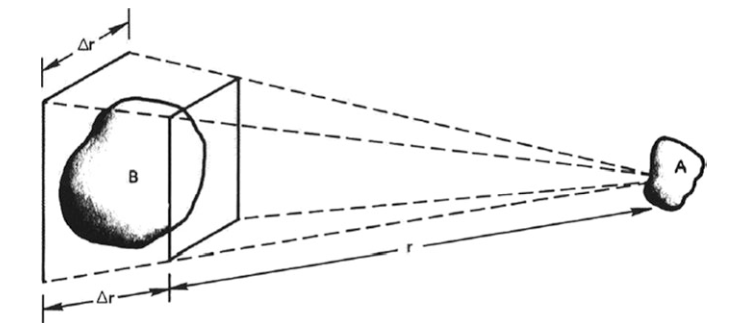
\includegraphics[width=0.7\linewidth]{solid_angle.png}
  \caption{遠距離に作用するクーロン力}
  \label{fig:sample}
\end{figure}


\subsection{温度の概念}
先に進む前に、温度の物理的な概念を見直そう。熱平衡状態の気体の速度分布はマクスウェル分布

\section{結論}
LaTeXを使えば、美しい日本語の文書を作成することができます。ぜひ活用してみてください。




\begin{thebibliography}{99}
\bibitem{a} Francis F. Chen, Introduction to Plasma Physics and Controlled Fusion, Springer; Softcover reprint of the original 3rd ed., 2019\par
\url{http://library.unisel.edu.my/equip-unisel/custom/ebook_catalog/2016BookIntroductionToPlasmaPhysicsAndcompressed.pdf}
\bibitem{b} 宮本健郎, プラズマ物理の基礎, 朝倉書店 , 2014\par
\url{https://op.lib.kobe-u.ac.jp/opac/opac_details/?reqCode=fromlist&lang=0&amode=11&bibid=2002133568&opkey=B175679900718865&start=1&totalnum=4&listnum=1&place=&list_disp=20&list_sort=0&cmode=0&chk_st=0&check=0000}
\bibitem{c} EMANの物理学\par
\url{https://eman-physics.net/electromag/plasma.html}
\end{thebibliography}





\end{document}